% Created 2022-07-03 Sun 20:44
% Intended LaTeX compiler: pdflatex
% made in emacs org-mode and then exported to TeX
\documentclass[11pt]{article}
\usepackage[utf8]{inputenc}
\usepackage[T1]{fontenc}
\usepackage{graphicx}
\usepackage{longtable}
\usepackage{wrapfig}
\usepackage{rotating}
\usepackage[normalem]{ulem}
\usepackage{amsmath}
\usepackage{amssymb}
\usepackage{capt-of}
\usepackage{hyperref}
\author{Ethan Goan}
\date{\today}
\title{ProbML Reading Group - Challenge 4.1}
\hypersetup{
 pdfauthor={Ethan Goan},
 pdftitle={ProbML Reading Group - Challenge 4.1},
 pdfkeywords={},
 pdfsubject={},
 pdfcreator={Emacs 28.1 (Org mode 9.6)},
 pdflang={English}}
\usepackage{biblatex}
\usepackage{tikz}
\usetikzlibrary{bayesnet}
\usepackage{array}
\newcommand{\PreserveBackslash}[1]{\let\temp=\\#1\let\\=\temp}
\newcolumntype{C}[1]{>{\PreserveBackslash\centering}p{#1}}
\newcolumntype{R}[1]{>{\PreserveBackslash\raggedleft}p{#1}}
\newcolumntype{L}[1]{>{\PreserveBackslash\raggedright}p{#1}}
\newcommand\independent{\protect\mathpalette{\protect\independenT}{\perp}}
\def\independenT#1#2{\mathrel{\rlap{$#1#2$}\mkern2mu{#1#2}}}
\addbibresource{~/.local/ref.bib}
\begin{document}

\maketitle


\section{The Model}
\label{sec:org5b48f49}
We are given a model such that,
\[ p(w,x,y,z) = p(w)p(x|w)p(z|x)p(y|x) \]
% Simple Bayesian network
and we are tasked with creating a new model from this using the principles of Bayes' Rule, where the new model is,

\[ p(w,x,y,z) = p(w)p(y)p(x|w,y)p(z|x). \]

First lets plot these models.
\begin{figure}[!h]
  \begin{center}
    \begin{tabular}{L{5cm}R{5cm}}
      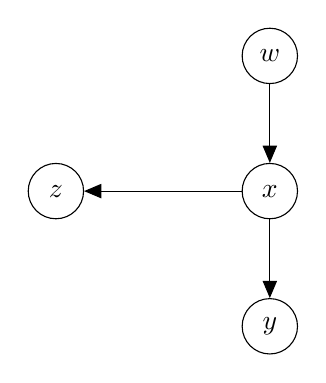
\begin{tikzpicture}

  % Define nodes
  \node[latent]                               (w) {$w$};
  \node[latent, below=of w] (x) {$x$};
  \node[latent, below=of x] (y) {$y$};
  \node[latent, left=2cm of x]            (z) {$z$};

  % Connect the nodes
  \edge {w} {x} ; %
  \edge {x} {y,z} ; %
\end{tikzpicture}
%%% Local Variables:
%%% mode: latex
%%% TeX-master: t
%%% End:
 &
      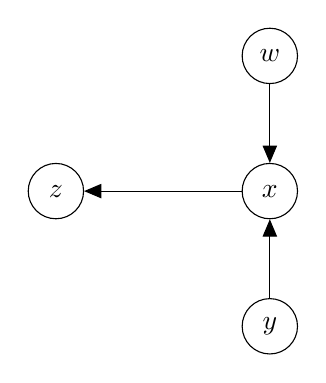
\begin{tikzpicture}

  % Define nodes
  \node[latent]                               (w) {$w$};
  \node[latent, below=of w] (x) {$x$};
  \node[latent, below=of x] (y) {$y$};
  \node[latent, left=2cm of x]            (z) {$z$};

  % Connect the nodes
  \edge {w} {x} ; %
  \edge {x} {z} ; %
  \edge {y} {x} ; %
\end{tikzpicture}
%%% Local Variables:
%%% mode: latex
%%% TeX-master: t
%%% End:

      \\
      \\
      Original Model & New Model
    \end{tabular}
  \end{center}
  \caption{Our original model on the left and the new model on the right, where the direction between variables $x$ and $y$ is reversed.}
\end{figure}


What we want to do is to reverse the arrow between \(x\) and \(y\) using Bayes' Rule.

\subsection{Being Good Bayesian's}
Recap of Bayes' Rule,
\[ p(\theta | t)  =  \frac{p(\theta) p(t | \theta)}{p(t)}\]

To replace the direction between \(x\) and \(y\) will change what we are conditioning on and our marginal distributions, such that we will be replacing
\(p(y|x)\) with \(p(y)\), and our conditional distribution for \(x\) will now include a term for \(y\) \(p(x | w, y)\).

\begin{align*}
p(y) &= \sum_{w,x,z} p(w,x,y,z)
\\
 & = \sum_{w,x,z} \underbrace{p(y|w,x,z)p(w,x,z)}_{\text{product rule}}
\\
 & = \sum_{w,x,z} \underbrace{p(y|x)p(x,w,z)}_{\text{product rule + graph structure}}
\\
 & = \sum_{w,x,z} p(y|x) p(w) p(x|w)p(z|x)
\end{align*}

Can now separate some of the summation terms exploiting the properties of conditional independence in our graph.

\begin{align*}
p(y) & = \sum_{x,z} p(y|x) p(z|x) \underbrace{\sum_{w} p(w)p(x|w)}_{p(x)}
\\
& = \sum_{x} p(y|x) p(x) \sum_{z} p(z|x)
\\
& = \Big( \sum_{x} p(y|x) p(x) \Big) \Big( \sum_{x} p(x) \underbrace{\sum_{z} p(z|x)}_{=1} \Big)
\\
& = \Big(\sum_{x} p(y|x) p(x) \Big) \Big(\underbrace{\sum_{x} p(x)}_{=1} \Big)
\\
& = \sum_{x} p(y|x) p(x) = p(y)
\end{align*}


\subsection{How does this effect the conditional independence of our variables?}
\label{sec:orgae8a6b8}
Conditional independence between variables \(A\) and \(B\) given \(C\) can be described as,
\[ p(A, |B ,C ) = p(A | C) \]

Want to see how conditional independence is effected given the change in our graph structure.

\subsubsection{Conditional Independence between \(z\) and \(y\) given \(x\)}
\begin{align*}
p(z |x, y)_{\text{graph one}} &= \frac{\sum_{w}p(w)p(x | w)p(z | x)  p(y | x)} {\sum_{z,w} p(w)p(z | x) p(x | w) p(y | x)}
\\
&= \frac{p(x) p(z | x)  p(y | x)} { p(y | x)}
\\
&= p(x) p(z | x)
\end{align*}

When moving to our new graph,

\begin{align*}
p(z | x, y)_{\text{graph two}} &= \frac{\sum_{w}p(z | x)p(x | w, y) p(y)   p(w) } {\sum_{w,z}p(z | x) p(w) p(x | w, y) p(y)}
\\
&= \frac{p(z | x) p(y)  p(x | y) } { p(x|y) p(y)}
\\
&= p(z | x)
\end{align*}

They remain conditionally dependent in both cases.



\subsubsection{Conditional Independence between \(w\) and \(y\)  given \(x\)}
In our original graph,
\begin{align*}
p(y | w, x)_{\text{graph one}} &= \frac{\sum_{z}p(z | x) p(w) p(x | w) p(y | x)} {\sum_{y,z}p(z | x) p(w) p(x | w) p(y | x)}
\\
&= \frac{ p(w) p(x | w) p(y | x)} { p(w) p(x | w)}
\\
&= p(y | x)
\end{align*}
Therefore \(y \independent w | x\).


When moving to our new graph,

\begin{align*}
p(y | w, x)_{\text{graph two}} &= \frac{\sum_{z}p(z | x) p(w) p(x | w, y) p(y) } {\sum_{y,z}p(z | x) p(w) p(x | w, y) p(y)}
\\
&= \frac{p(w) p(x | w, y) p(y) } { p(w) p(x | w)}
\\
&= \frac{p(x | w, y) p(y) } { p(x | w)}
\end{align*}
\(y\)  and \(w\) are no longer conditionally independent given \(x\).
%
%
\newline
Probability is pretty dang cool.
\end{document}
%%% Local Variables:
%%% mode: latex
%%% TeX-master: t
%%% End:
